\documentclass[10pt,a4paper]{article}
\usepackage{amsmath}
\usepackage{amssymb}
\usepackage{graphicx}
\usepackage{color}
\usepackage{fancyhdr}
\usepackage{fancyvrb}
\usepackage[margin=3.5cm]{geometry}
\usepackage{framed}
\usepackage{enumerate}
\usepackage{textcomp}
\def\ket#1{\left|#1\right\rangle}
\def\bra#1{\left\langle#1\right|}
\def\braket#1{\left\langle#1\right\rangle}

\definecolor{linkcol}{rgb}{0.0, 0.0, 0.7}
\usepackage[colorlinks=true,urlcolor=linkcol,citecolor=black,linkcolor=linkcol]{hyperref}

\renewcommand{\theequation}{8.\arabic{equation}}
\setcounter{section}{8}
\renewcommand\thesection{\arabic{section}}
\renewcommand\thesubsection{\thesection.\arabic{subsection}}

\fancyhf{}
\lhead{\tiny Y.~D.~Chong (2021)}
\rhead{\scriptsize MH2801: Complex Methods for the Sciences}
\lfoot{}
\rfoot{\thepage}
\pagestyle{fancy}

\begin{document}
\setcounter{page}{54}

\noindent
{\Large \textbf{8. Mathematical Functions}}
\vskip 0.2in

\label{branch-points-and-branch-cuts}

When introducing complex algebra in Chapter 4, we postponed discussion
of what it means to raise a complex number to a non-integer power,
such as $z^{1/2}$, $z^{4/3}$, or $z^{\pi}$. It is now time to open
that can of worms.

\subsection{Non-integer powers as multi-valued operations}
\label{non-integer-powers-as-multi-valued-operations}

Given a complex number in its polar representation, $z = r
e^{i\theta}$, raising to the power of $p$ could be handled this way:
\begin{align}
  z^p = \left(re^{i\theta}\right)^p = r^p e^{ip\theta}.
\end{align}
Let's take a closer look at the complex exponential term
$e^{ip\theta}$.  Since $\theta = \mathrm{arg}(z)$ is an angle, we can
change it by multiples of $2\pi$ without altering the value of $z$.
So we can re-write the above equation as
\begin{align}
  z^p = \left(r\,e^{i(\theta + 2\pi n)}\right)^p = \left(r^p e^{ip\theta} \right) e^{2\pi i n p}, \quad \mathrm{where}\;\; n\in\mathbb{Z}.
\end{align}
If $p$ is an integer, this re-statement is somewhat trivial: no matter
what integer $n$ we take, $2\pi n p$ is a multiple of $2\pi$, so $z^p$
ends up with the same value:
\begin{align}
  z^p = r^p e^{ip\theta} \;\;\textrm{unambiguously} \;\;\;(\text{if}\;p\in\mathbb{Z}).
\end{align}
But if $p$ is not an integer, the $\exp\left(2 \pi i np\right)$ factor
takes on different values for different $n$. In that case, the ``power
of $p$'' is a \textbf{multi-valued operation}. It cannot be treated as
a function in the usual sense, since functions must have unambiguous
outputs.

\subsection{Roots of unity}\label{roots-of-unity}

Let's take a closer look at the problematic exponential term,
\begin{align}
  \exp\left(2\pi i np\right), \quad\mathrm{where}\;\; n \in \mathbb{Z}.
\end{align}
If $p$ is irrational, $2\pi np$ never repeats modulo $2\pi$. Thus,
$z^p$ has an infinite set of values, one for each integer $n$.

More interesting is the case of a non-integer \textit{rational}
power. Any rational number can be written as $p = P/Q$ where $P$ and
$Q$ are integers with no common divisor.  It can be proven using
modular arithmetic (though we will not go into the details) that $2\pi
n\, (P/Q)$ has exactly $Q$ unique values modulo $2\pi$:
\begin{align}
  2 \pi n p = 2\pi n\, \left(\frac{P}{Q}\right) = 2\pi \times \left\{0,\, \frac{1}{Q},\, \frac{2}{Q},\, \dots, \frac{(Q-1)}{Q} \right\} \quad(\mathrm{modulo} \; 2\pi).
\end{align}
The set of values is independent of the numerator $P$.  The value of
$P$ merely affects the sequence in which the numbers are generated as
we step though the integer values of $n$. This is demonstrated by the
following examples:

\begin{framed} \noindent
\textit{Example}---Consider the complex square root operation,
$z^{1/2}$. If we write $z$ in its polar respresentation, $z = r
e^{i\theta}$, then
\begin{equation}
  z^{1/2} = \left[r \, e^{i(\theta + 2 \pi n)} \right]^{1/2} = r^{1/2} \, e^{i\theta/2} \, e^{i \pi n}, \quad n \in \mathbb{Z}.
\end{equation}
The $e^{i\pi n}$ factor has two possible values: $+1$ (for even $n$) and $-1$ (for odd $n$). Hence, the values of the square root are
\begin{equation}
  z^{1/2} = r^{1/2} \, e^{i\theta/2} \;\times\; \left\{1, -1\right\}.
\end{equation}
\end{framed}

\begin{framed} \noindent
  \textit{Example}---Consider the cube root operation $z^{1/3}$.
  Taking $z = r e^{i\theta}$, we obtain
\begin{equation}
z^{1/3} = r^{1/3} \, e^{i\theta/3} \, e^{2\pi i n/3}, \quad n \in \mathbb{Z}.
\end{equation}
Running through $n$ gives
\begin{align*}
  \begin{array}{|c||c|c|c|c|c|c|c|c|c|} \hline n &\cdots & -2 & -1 & 0 & 1 & 2 & 3 & 4 & \cdots \\ \hline 2\pi n / 3 &\cdots & -4\pi/3 & -2\pi/3 & 0 & 2\pi/3 & 4\pi/3 & 6\pi/3 & 8\pi/3 & \cdots \\ \hline e^{2\pi i n/3} &\cdots & e^{2\pi i /3} & e^{-2\pi i /3} & \;\,\;1\;\,\; & e^{2\pi i /3} & e^{-2\pi i /3} & \;\,\;1\;\,\; & e^{2\pi i /3} & \cdots \\ \hline \end{array}
\end{align*}
Hence, the cube root operation has three distinct values:
\begin{equation}
  z^{1/3} = r^{1/3} \, e^{i\theta/3} \;\times\; \left\{\;
  1, \;e^{2\pi i /3},\; e^{-2\pi i /3}\; \right\}.
\end{equation}
\end{framed}

%% \vskip 0.15in

\begin{framed} \noindent
  \textit{Example}---Consider the operation $z^{2/3}$. Again taking
  $z = re^{i\theta}$,
\begin{equation}
  z^{2/3} = r^{2/3} \, e^{2i\theta/3} \, e^{4\pi i n/3}, \quad n \in \mathbb{Z}.
\end{equation}
Running through $n$ gives
\begin{align*}
  \begin{array}{|c||c|c|c|c|c|c|c|c|c|} \hline n &\cdots & -2 & -1 & 0 & 1 & 2 & 3 & 4 & \cdots \\ \hline 4\pi n / 3 &\cdots & -8\pi/3 & -4\pi/3 & 0 & 4\pi/3 & 8\pi/3 & 12\pi/3 & 16\pi/3 & \cdots \\ \hline e^{4\pi i n/3} &\cdots & e^{-2\pi i /3} & e^{2\pi i /3} & \;\,\;1\;\,\; & e^{-2\pi i /3} & e^{2\pi i /3} & \;\,\;1\;\,\; & e^{-2\pi i /3} & \cdots \\ \hline \end{array}
\end{align*}
Hence,
\begin{equation}
z^{2/3} = r^{2/3} \, e^{2i\theta/3} \;\times\; \left\{\;1,\; e^{2\pi i /3},\; e^{-2\pi i /3}\;\right\}.
\end{equation}
Note that the set of values in curly brackets is the same as in the
previous example, demonstrating that the numerator $P$ does not affect
the set.
\end{framed}

\vskip 0.2in

From the above examples, we deduce the following expression for rational powers:
\begin{align}
  z^{P/Q} = r^{P/Q} \; e^{i\theta\, (P/Q)}\, \times \Big\{1,\, e^{2\pi i /Q},\, e^{4\pi i /Q},\, \dots, e^{2\pi i (1-Q)/Q} \Big\}.
\end{align}
The quantities in the curly brackets are called the \textbf{roots of
  unity}. In the complex plane, they sit at $Q$ evenly-spaced points
on the unit circle, with $1$ as one of the values:

\vskip 0.2in
\begin{figure}[ht]
  \centering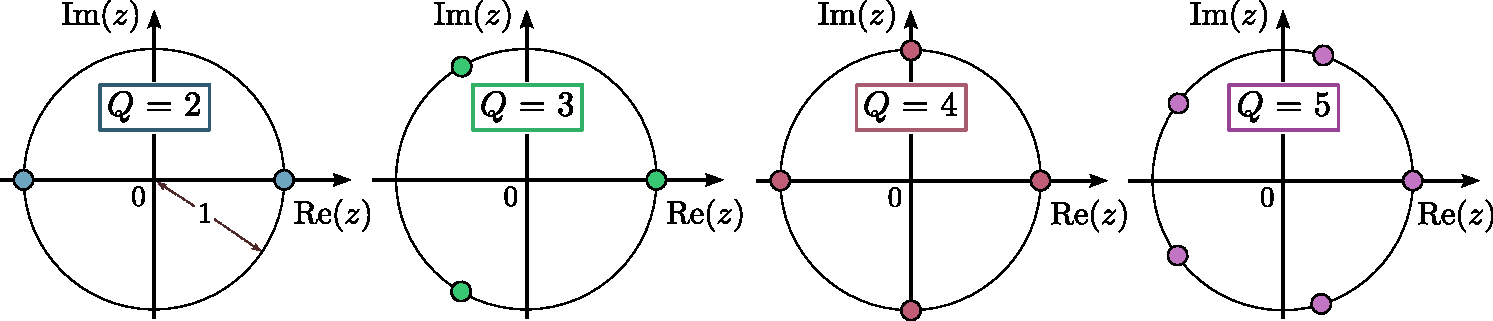
\includegraphics[width=0.99\textwidth]{roots_of_unity}
\end{figure}

\clearpage

\subsection{Complex logarithms}\label{complex-logarithms}

Here is another way to think about non-integer powers.  Recall what it
means to raise a number to, say, the power of 5: we simply multiply
the number by itself five times.  What about raising a number to a
non-integer power $p$?  For the real case, the power is defined as a
combination of exponential and logarithm functions, as we saw in
Section 0.2:
\begin{align}
  x^p \equiv \exp\!\big[\,p\ln(x)\big].
\end{align}
This definition relies on the fact that, for real inputs, the
logarithm is a well-defined function.  That, in turn, comes from the
definition of the logarithm as the inverse of the exponential
function. Since the real exponential is one-to-one, its inverse is
also one-to-one.

The complex exponential, however, is many-to-one, since changing its
input by any multiple of $2\pi i$ yields the same output:
\begin{align}
  \exp(z + 2\pi i n) = \exp(z) \cdot e^{2\pi i n} = \exp(z) \quad \mathrm{for~all}\;\, n \in \mathbb{Z}.
\end{align}
The inverse of the complex exponential is the \textbf{complex
  logarithm}. Since the complex exponential is many-to-one, the
complex logarithm is one-to-many.  For each $z$, there is an infinite
set of values for $\ln(z)$, separated by integer multiples of $2\pi
i$:
\begin{align}
  \ln(z) = \big[\ln(z)\big]_{\mathrm{p.v.}}\, +\; 2 \pi i n, \quad n \in \mathbb{Z}.
\end{align}
Here, $[\ln(z)]_{\mathrm{p.v.}}$ denotes the \textbf{principal value}
of $\ln(z)$, which refers to a reference value of the logarithm
operation (which we'll define later).  Do not think of the principal
value as the ``actual'' result of the $\ln(z)$ operation! There are
multiple values, each equally legitimate; the principal value is
merely one of them.

We now apply the formula $z^p \equiv \exp\left[p\ln(z)\right]$, with
$\ln(z)$ as the multi-valued complex logarithm. Then
\begin{align}
  z^p &= \exp\Big\{p\big(\big[\ln(z)\big]_{\mathrm{p.v.}} + 2\pi i n\big)\Big\}\\
  &= \exp\Big\{p\,\big[\ln(z)\big]_{\mathrm{p.v.}}\Big\} \; e^{2\pi i np}, \quad n \in \mathbb{Z}\\
  &= \big[\,z^p\,\big]_{\mathrm{p.v.}} \; e^{2\pi i np}, \quad\qquad\qquad\;\;\, n \in \mathbb{Z}.
\end{align}
The factor of $e^{2\pi i np}$, which is responsible for the
multi-valuedness, corresponds to the roots of unity discussed in
Section~\ref{roots-of-unity}.

\subsection{Branches}\label{branches}

We have discussed two examples of multi-valued complex operations:
non-integer powers and the complex logarithm. However, we usually
prefer to deal with functions rather than multi-valued operations. One
reason is that the concept of the complex derivative is based on
functions, not multi-valued operations.

There is a standard procedure to convert multi-valued operations into
functions. First, we define one or more curve(s) in the complex plane,
called \textbf{branch cuts} (the reason for this name will be
explained later).  Next, we modify the domain (i.e., the set of
permissible inputs) by excluding all values of $z$ lying on a branch
cut. Then the outputs of the multi-valued operation can be grouped
into discrete \textbf{branches}, each behaving as a function.

The above procedure can be understood through the example of the
square root.

\subsubsection{Branches of the complex square root}
\label{branches-of-the-complex-square-root}

We saw in Section~\ref{roots-of-unity} that the complex square root,
$z^{1/2}$, has two possible values. We can define the two branches as
follows:

\begin{enumerate}
\item Define a branch cut along the negative real axis, so that the
  domain excludes all $z$ along the branch cut. In other words, we
  will only consider complex numbers whose polar representation can be
  written as $$z = r e^{i\theta}, \quad \theta \in (-\pi, \pi).$$ (For
  those unfamiliar with this notation, $\theta \in (-\pi, \pi)$ refers
  to the interval $-\pi < \theta < \pi$.  The parentheses indicate
  that the boundary values of $-\pi$ and $\pi$ are excluded.  By
  contrast, we would write $\theta \in [-\pi, \pi]$ to refer to the
  interval $-\pi \le \theta \le \pi$, with the square brackets
  indicating that the boundary values are included.)

\item One branch is associated with the root of unity $+1$. On this
  branch, for $z = re^{i\theta}$, the value is $$f_+(z) = r^{1/2} \,
  e^{i\theta/2}, \quad \theta \in (-\pi, \pi).$$

\item The other branch is associated with the root of unity $-1$. On
  this branch, the value is $$f_-(z) = -r^{1/2} \, e^{i\theta/2},
  \quad \theta \in (-\pi, \pi).$$
\end{enumerate}

\noindent
The following plot shows how varying $z$ affects the positions of
$f_+(z)$ and $f_-(z)$ in the complex plane:

\begin{figure}[h]
  \centering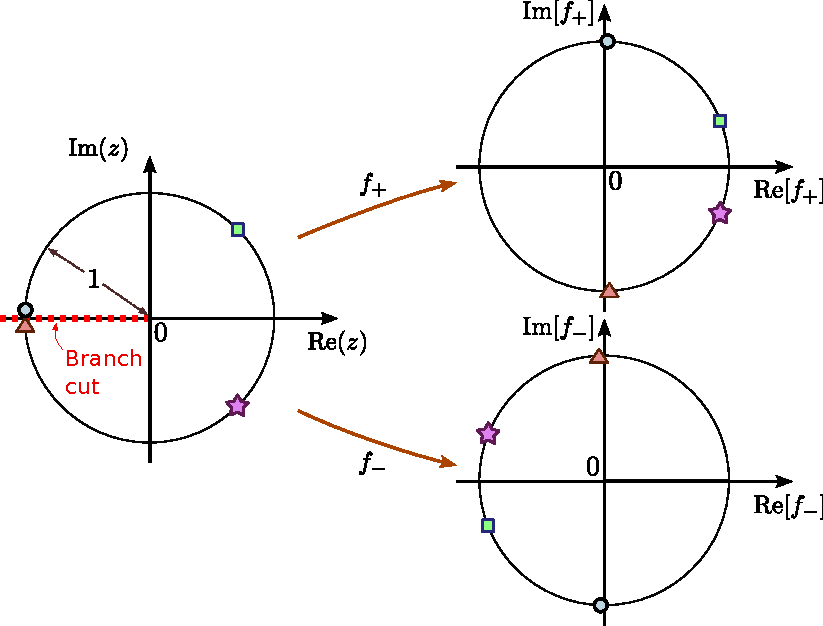
\includegraphics[width=0.75\textwidth]{complex_root_1}
\end{figure}

\noindent
In the left subplot, the red dashes indicate the branch cut, and the
various symbols (circle, square, star, and triangle) indicate
representative values of $z$.  In the right subplots, the symbols
indicate the corresponding positions of $f_+(z)$ and $f_-(z)$ in the
complex plane.

Note that $f_+(z)$ always lies in the right half of the complex plane,
whereas $f_-(z)$ lies in the left half of the complex plane. Both
$f_+$ and $f_-$ are well-defined functions with unambiguous outputs,
albeit with domains that do not cover the entire complex plane (i.e.,
the branch cut is excluded).

It can moreover be shown that these functions are analytic over all of
the complex plane except the branch cut (see Section 6.2); this can be
proven using the Cauchy-Riemann equations, and is left as an exercise.

The end-point of the branch cut is called a \textbf{branch point}. For
$z = 0$, both branches give the same result: $f_+(0) = f_-(0) = 0$. We
will have more to say about branch points in
Section~\ref{branch-points}.

\subsubsection{Different branch cuts for the complex square root}
\label{different-branch-cuts-for-the-complex-square-root}

You may be wondering why the branch cut has to lie along the negative
real axis. In fact, this choice is not unique. For instance, we could
place the branch cut along the positive real axis. This corresponds to
specifying the input $z$ using a different interval for $\theta$:
\begin{align}
  z = re^{i\theta}, \quad \theta \in (0, 2\pi).
\end{align}
Next, we use the same formulas as before to define the branches of the
complex square root:
\begin{align}
  f_\pm(z) = \pm r^{1/2} \, e^{i\theta/2}.
\end{align}
But because the domain of $\theta$ has been changed to $(0, 2\pi)$,
the set of inputs $z$ now excludes the positive real axis. With this
new choice of branch cut, the values produced by the branch functions
are shown in the following figure:

\begin{figure}[h]
  \centering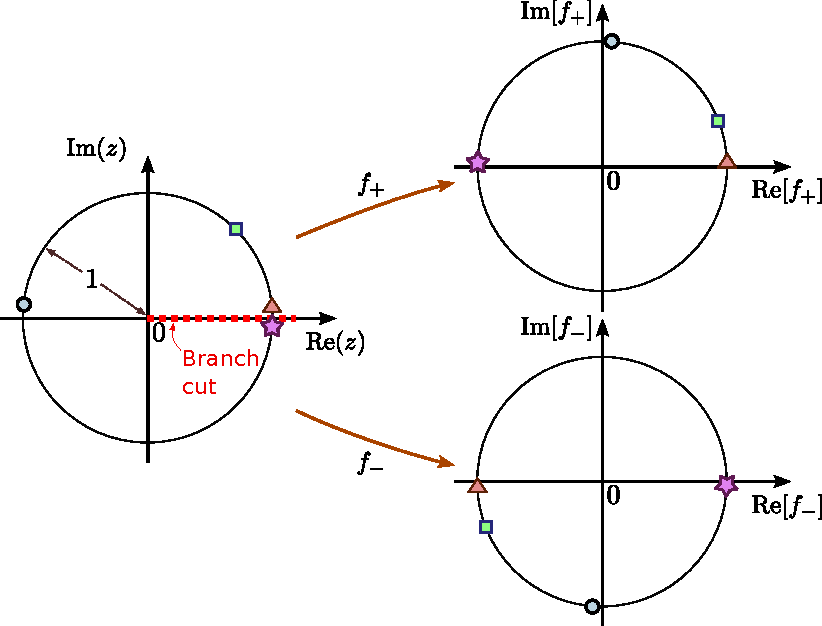
\includegraphics[width=0.75\textwidth]{complex_root_2}
\end{figure}

The two branch functions are different from what we had before.  Now,
$f_+(z)$ is always in the upper half of the complex plane, and
$f_-(z)$ in the lower half of the complex plane. However, both
branches still have the same value at the branch point: $f_+(0) =
f_-(0) = 0$.

We can think of the branch cut as a boundary where two branches are
``glued'' together, so that crossing the branch cut brings us from one
branch to a different branch.  For example, in the left subplot,
consider the value of $z$ indicated by the triangle, which lies just
above the branch cut.  In the right subplots, observe that the
corresponding value of $f_+(z)$ lies just above the positive real
axis, and $f_-(z)$ lies just below the negative real axis.

Next, consider the value of $z$ indicated by the star, which lies just
below the branch cut.  Going from the triangle to the star is
equivalent to a small downwards displacement of $z$, ``crossing'' the
branch cut.  Now the values of the positive and negative branches are
swapped: $f_-(z)$ lies just below the positive real axis, near where
$f_+(z)$ was previously, and $f_+(z)$ now lies just above the negative
real axis where $f_-(z)$ was previously.

The three-dimensional plot below provides another way to visualize the
role of the branch cut.  Here, the horizontal axes correspond to $x =
\mathrm{Re}(z)$ and $y = \mathrm{Im}(z)$. The vertical axis shows the
arguments for the two values of the complex square root, with
$\mathrm{arg}\big[f_+(z)\big]$ plotted in orange and
$\mathrm{arg}\big[f_-(z)\big]$ plotted in blue. The choice of branch
cut, shown as a red line, is just a choice about how to divide up the
branches of a multi-valued operation.

\begin{figure}[h]
  \centering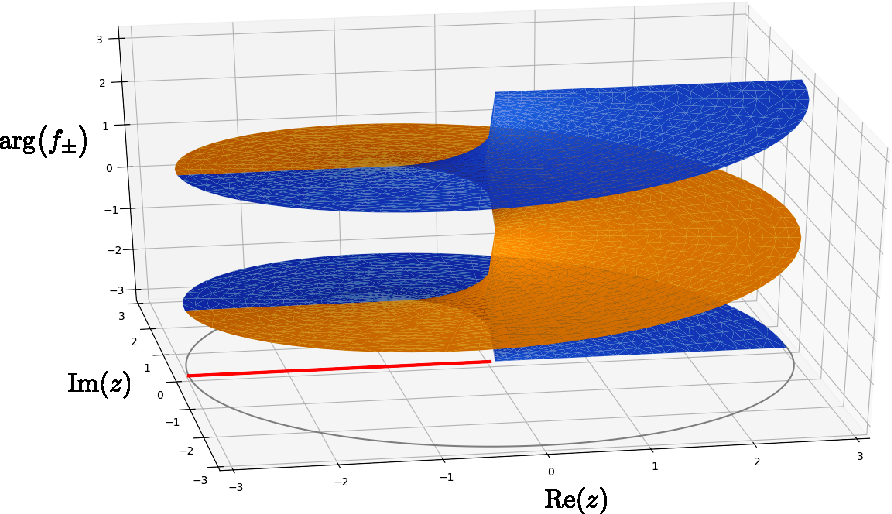
\includegraphics[width=0.7\textwidth]{branches}
\end{figure}

\subsubsection{Branch points}
\label{branch-points}

The tip of each branch cut is called a \textbf{branch point}. A branch
point is a point where different branches have the same value. Whereas
the choice of branch cuts is non-unique, the branch points of a
multi-valued operation are uniquely determined.

For the purposes of this course, you mostly only need to remember the
branch points arising from two common cases:

\begin{itemize}
\item The $z^p$ operation (for non-integer $p$) has branch points at
  $z = 0$ and $z = \infty$.

\item The complex logarithm has branch points at $z = 0$ and $z = \infty$.
\end{itemize}

\noindent
We can easily see that $z^p$ must have a branch point at $z = 0$: at
this point, the value has to be $0$, regardless of the choice of root
of unity. As for the branch point at $z = \infty$, understanding it
requires us to know more about the concept of ``infinity'' for complex
numbers.

\subsection{The meaning of ``infinity'' for complex numbers (optional topic)}
\label{aside-the-meaning-of-infinity-for-complex-numbers}

When talking about the \textbf{complex infinity}, $z = \infty$, we are
referring to a complex number with infinite magnitude and
\textit{undefined} argument.

The idea of a complex number having undefined argument may seem
strange, but actually we already know of another complex number with
this feature: $z = 0$ has zero magnitude and undefined argument.
These two special complex numbers are the reciprocals of each other:
$1/\infty = 0$ and $1/0 = \infty$.

The complex $\infty$ behaves differently from the familiar concept of
infinity associated with real numbers. For real numbers, positive
infinity ($+\infty$) is distinct from negative infinity
($-\infty$). But this doesn't hold for complex numbers, since complex
numbers occupy a two-dimensional plane rather than a line. Thus, for
complex numbers it does not make sense to define ``positive infinity''
and ``negative infinity'' as distinct entities.

From this, we can see why $z^p$ has a branch point at $z =
\infty$. For any finite and nonzero $z$, we can write $z =
re^{i\theta}$, where $r$ is a positive number. The values of the $z^p$
operation have the form
\begin{align}
  r^p \, e^{ip\theta}\,\times\, \{\text{roots of unity}\}.
\end{align}
Regardless of which root of unity we pick, the magnitude is $r^p$; as
$r \rightarrow \infty$, the magnitude goes to infinity and the overall
complex value goes to $\infty$. Hence, at $z = \infty$ all the
branches of $z^p$ have the same value (i.e., $\infty$).

By similar reasoning, one can prove that $\ln(z)$ has branch points at
$z = 0$ and $z = \infty$.  This is left as an exercise.

\subsection{Branch cuts for general multi-valued operations}
\label{branch-cuts-for-general-multi-valued-operations}

Having discussed the simplest multi-valued operations, $z^p$ and
$\ln(z)$, here is how to assign branch cuts for more general
multi-valued operations. This is a two-step process:

\begin{enumerate}
\item Locate the branch points.

\item Assign branch cuts in the complex plane, such that (i) every
  branch point has a branch cut ending on it, and (ii) every branch
  cut ends on a branch point. The branch cuts should not intersect.
\end{enumerate}

\noindent
The choice of where to place branch cuts is not unique.  Branch cuts
are usually chosen to be straight lines, for simplicity, but this is
not necessary. Different choices of branch cuts correspond to
different ways of partitioning the values of the multi-valued
operation into separate branches.

\subsubsection{An important example}
\label{an-important-example}

We can illustrate the process of assigning branch cuts, and defining
branch functions, with the following multi-valued operation:
\begin{align}
  f(z) = \ln\left(\frac{z+1}{z-1}\right).
\end{align}
This is multi-valued because of the presence of the complex
logarithm. The branch points are $z = 1$ and $z = -1$, as these are
the points where the input to the logarithm becomes $\infty$ or $0$
respectively. Note that $z = \infty$ is \textit{not} a branch point;
at $z = \infty$, the input to the logarithm is $-1$, which is not a
branch point for the logarithm.

We can assign any branch cut that joins the branch points at $z = \pm
1$.  A convenient choice is shown below:

\begin{center}
  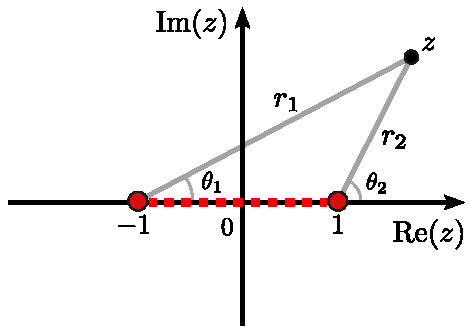
\includegraphics[width=0.4\textwidth]{branch_cut_example}
\end{center}

This choice of branch cut is nice because we can express the $z+1$ and
$z - 1$ terms using the polar representations
\begin{align}
  z + 1 &= r_1\,e^{i\theta_1}, \\
  z - 1 &= r_2\, e^{i\theta_2},
\end{align}
where $r_1$, $r_2$, $\theta_1$, and $\theta_2$ are shown graphically
in the above figure. The positioning of the branch cut corresponds to
a particular choice for the ranges of the complex arguments $\theta_1$
and $\theta_2$.  As we'll shortly see, the present choice of branch
cut corresponds to
\begin{align}
  \theta_1 \in (-\pi,\pi), \quad \theta_2 \in (-\pi,\pi).
\end{align}
Hence, $f(z)$ can be written as
\begin{align}
  f(z) = \ln\left(\frac{r_1}{r_2}\right) + i(\theta_1 - \theta_2 + 2\pi m), \;\;\mathrm{where}\;\;\;\left\{\begin{aligned} m &\in\mathbb{Z},\\ z &= -1 + r_1\,e^{i\theta_1} = 1 + r_2\,e^{i\theta_2},\\ \theta_1, \theta_2 &\in (-\pi,\pi).\end{aligned}\right.
\end{align}
The choice of $m$ specifies the branch, and we can choose $m = 0$ as
the principal branch.

Let us verify that setting $\theta_1 \in (-\pi,\pi)$ and $\theta_2 \in
(-\pi,\pi)$ is consistent with our choice of branch cut. Consider the
principal branch, and compare the outputs of the above formula for $z$
just above the real axis, and for $z$ just below the real axis.  There
are three cases of interest, depending on $\mathrm{Re}[z]$:

Firstly, for $\mathrm{Re}[z] < -1$ (to the left of the leftmost branch
point),
\begin{align}
  \mathrm{Im}[z] &= 0^+ \Rightarrow\; \theta_1 \rightarrow \pi, \;\;\; \theta_2 \rightarrow \pi\;\;\;\;\,\Rightarrow\; f(z) = \ln\!\left(\frac{r_1}{r_2}\right) + i\big((\pi) - (\pi)\big) \quad\;\; = \ln\left(\frac{r_1}{r_2}\right) \\
  \mathrm{Im}[z] &= 0^- \Rightarrow\; \theta_1 \rightarrow -\pi, \; \theta_2 \rightarrow -\pi \;\Rightarrow \; f(z) = \ln\!\left(\frac{r_1}{r_2}\right) + i\big((-\pi) - (-\pi)\big) = \ln\left(\frac{r_1}{r_2}\right)
\end{align}
(If you're not sure why $\theta_1$ and $\theta_2$ have these values,
look carefully at the above figure, and think about what values
$\theta_1$ and $\theta_2$ would have for, say, $z = -2 + 0.001i$ or $z
= -2 - 0.001i$.) Thus, there is no discontinuity along this segment of
the real axis.

Secondly, for $-1 < \mathrm{Re}[z] < 1$ (between the two branch
points),
\begin{align}
  \mathrm{Im}[z] &= 0^+ \Rightarrow \theta_1 \rightarrow 0, \; \theta_2 \rightarrow \pi \;\;\;\Rightarrow\; f(z) = \ln\!\left(\frac{r_1}{r_2}\right) + i\big((0) - (\pi)\big) \;\;\,= \ln\left(\frac{r_1}{r_2}\right) -i\pi \\
  \mathrm{Im}[z] &= 0^- \Rightarrow \theta_1 \rightarrow 0, \; \theta_2 \rightarrow -\pi \,\Rightarrow\; f(z) = \ln\!\left(\frac{r_1}{r_2}\right) + i\big((0) - (-\pi)\big) = \ln\left(\frac{r_1}{r_2}\right) + i\pi
\end{align}
Hence, in the segment between the two branch points, there is a
discontinuity of $\pm 2\pi i$ on different sides of the real axis.
The value of this discontinuity is exactly equal, of course, to the
separation between the different branches of the complex logarithm.

Finally, for $\mathrm{Re}[z] > 1$ (to the right of the rightmost
branch point), there is again no discontinuity:
\begin{align}
  \mathrm{Im}[z] &= 0^+ \Rightarrow \theta_1 \rightarrow 0, \; \theta_2 \rightarrow 0 \;\;\Rightarrow\;\; f(z) = \ln\!\left(\frac{r_1}{r_2}\right) + i\big((0) - (0)\big) = \ln\left(\frac{r_1}{r_2}\right) \\
  \mathrm{Im}[z] &= 0^- \Rightarrow \theta_1 \rightarrow 0, \; \theta_2 \rightarrow 0 \;\;\Rightarrow\;\; f(z) = \ln\!\left(\frac{r_1}{r_2}\right) + i\big((0) - (0)\big) = \ln\left(\frac{r_1}{r_2}\right).
\end{align}

\vskip 0.5in

\subsection{Exercises}\label{exercises}

\begin{enumerate}
\item
Find the values of $(i)^i$.
  \hfill{\scriptsize [solution~available]}

\item
Prove that $\ln(z)$ has branch points at $z = 0$ and $z = \infty$.
  \hfill{\scriptsize [solution~available]}

\item For each of the following multi-valued functions, find all the possible
function values, at the specified $z$:
\begin{enumerate}
\item $z^{1/3}$ at $z = 1$.

\item $z^{3/5}$ at $z = i$.

\item $\ln(z+i)$ at $z = 1$.

\item $\cos^{-1}(z)$ at $z = i$
\end{enumerate}

\item
For the square root operation $z^{1/2}$, choose a branch cut. Then
show that both the branch functions $f_\pm(z)$ are analytic over all
of $\mathbb{C}$ excluding the branch cut.

\item
  Consider $f(z) = \ln(z+a) - \ln(z-a)$. For simplicity, let $a$ be a
  positive real number. As discussed in
  Section~\ref{an-important-example}, we can write this as
\begin{equation}
f(z) = \ln\left|\frac{z+a}{z-a}\right| + i(\theta_+ - \theta_-), \qquad \theta_\pm \equiv \mathrm{arg}(z\pm a).
\end{equation}
Suppose we represent the arguments as $\theta_+ \in (-\pi,\pi)$ and
$\theta_- \in (-\pi,\pi)$. Explain why this implies a branch cut
consisting of a straight line joining $a$ with $-a$. Using this
representation, calculate the change in $f(z)$ over an infinitesimal
loop encircling $z = a$ or $z = -a$. Calculate also the change in
$f(z)$ over a loop of radius $R \gg a$ encircling the origin (and
thus enclosing both branch points).
\end{enumerate}
\end{document}
